% This example is meant to be compiled with lualatex or xelatex
% The theme itself also supports pdflatex
\PassOptionsToPackage{unicode}{hyperref}
\documentclass[aspectratio=1610, 12pt]{beamer}

% Warning, if another latex run is needed
% \usepackage[aux]{rerunfilecheck}

% just list chapters and sections in the toc, not subsections or smaller
\setcounter{tocdepth}{1}

%------------------------------------------------------------------------------
%------------------------------ Fonts, Unicode, Language ----------------------
%------------------------------------------------------------------------------
\usepackage{fontspec}
\defaultfontfeatures{Ligatures=TeX}  % -- becomes en-dash etc.

% german language
\usepackage{polyglossia}
\setdefaultlanguage{german}

% for english abstract and english titles in the toc
\setotherlanguages{english}

% intelligent quotation marks, language and nesting sensitive
\usepackage[autostyle]{csquotes}

% microtypographical features, makes the text look nicer on the small scale
\usepackage{microtype}

%------------------------------------------------------------------------------
%------------------------ Math Packages and settings --------------------------
%------------------------------------------------------------------------------

\usepackage{amsmath}
\usepackage{amssymb}
\usepackage{mathtools}
\usepackage{bbold}

% Enable Unicode-Math and follow the ISO-Standards for typesetting math
\usepackage[
  math-style=ISO,
  bold-style=ISO,
  sans-style=italic,
  nabla=upright,
  partial=upright,
]{unicode-math}
\setmathfont{Latin Modern Math}

% nice, small fracs for the text with \sfrac{}{}
\usepackage{xfrac}


%------------------------------------------------------------------------------
%---------------------------- Numbers and Units -------------------------------
%------------------------------------------------------------------------------

\usepackage[
  locale=DE,
  separate-uncertainty=true,
  per-mode=symbol-or-fraction,
]{siunitx}
\sisetup{math-micro=\text{µ},text-micro=µ}
% \sisetup{tophrase={{ to }}}
%------------------------------------------------------------------------------
%-------------------------------- tables  -------------------------------------
%------------------------------------------------------------------------------

\usepackage{booktabs}       % \toprule, \midrule, \bottomrule, etc

%------------------------------------------------------------------------------
%-------------------------------- graphics -------------------------------------
%------------------------------------------------------------------------------

\usepackage{graphicx}
%\usepackage{rotating}
\usepackage{grffile}
\usepackage{tikz}
\usepackage{circuitikz}
\usepackage{tikz-feynman}
\usepackage{subcaption}

% allow figures to be placed in the running text by default:
\usepackage{scrhack}
\usepackage{float}
\floatplacement{figure}{htbp}
\floatplacement{table}{htbp}

% keep figures and tables in the section
\usepackage[section, below]{placeins}

% smileys
\usepackage{MnSymbol,wasysym}

%------------------------------------------------------------------------------
%---------------------- customize list environments ---------------------------
%------------------------------------------------------------------------------

\usepackage{enumitem}
\usepackage{listings}
\usepackage{hepunits}

\usepackage{pdfpages}
%------------------------------------------------------------------------------
%------------------------------ Bibliographie ---------------------------------
%------------------------------------------------------------------------------

\usepackage[
  backend=biber,   % use modern biber backend
  autolang=hyphen, % load hyphenation rules for if language of bibentry is not
                   % german, has to be loaded with \setotherlanguages
                   % in the references.bib use langid={en} for english sources
]{biblatex}
\addbibresource{references.bib}  % the bib file to use
\DefineBibliographyStrings{german}{andothers = {{et\,al\adddot}}}  % replace u.a. with et al.


% Load packages you need here
% \usepackage{polyglossia}
% \setmainlanguage{german}

\usepackage{csquotes}


% \usepackage{amsmath}
% \usepackage{amssymb}
% \usepackage{mathtools}

\usepackage{hyperref}
\usepackage{bookmark}

% load the theme after all packages

\usetheme[
  showtotalframes, % show total number of frames in the footline
]{tudo}

% Put settings here, like
\unimathsetup{
  math-style=ISO,
  bold-style=ISO,
  nabla=upright,
  partial=upright,
  mathrm=sym,
}

% \setbeamertemplate{itemize item}{\scriptsize$\blacktriangleright$}
% \setbeamertemplate{itemize subitem}{\scriptsize$\blacktriangleright$}

%Titel:
\title{Understanding the alignment of LHCb's SciFi Tracker}
%Autor
\author[N.Breer]{Nils Breer*, Sophie Hollitt, Johannes Albrecht}
%Lehrstuhl/Fakultät
\institute{TU Dortmund, Fakultät Physik}
%Titelgrafik muss ich einfueren!!!
%\titlegraphic{\includegraphics[width=0.3\textwidth]{content/Bilder/interferenz.jpg}}
\date{13.03.2023}

\begin{document}
\maketitle

\begin{frame}\frametitle{Overview and Motivation}
$\textbf{Motivation}$
  \begin{itemize}
    \item $\bullet$\, Performance studies of alignments on run 256145 data
    \item \to\, unexpected different results!
    \item \to\, analysis of individual quarters
  \end{itemize}
$\textbf{Overview}$
  \begin{itemize}
    \item $\bullet$\, The SciFi Detector Upgrade
    \item $\bullet$\, Alignment how to
    \item $\bullet$\, Analysis of SciFi quarters in different alignment versions
  \end{itemize}
\end{frame}

\begin{frame}\frametitle{The Scintillating Fibre Tracker}
  \begin{columns}
    \begin{column}[c]{0.48\textwidth}
      \begin{figure}
        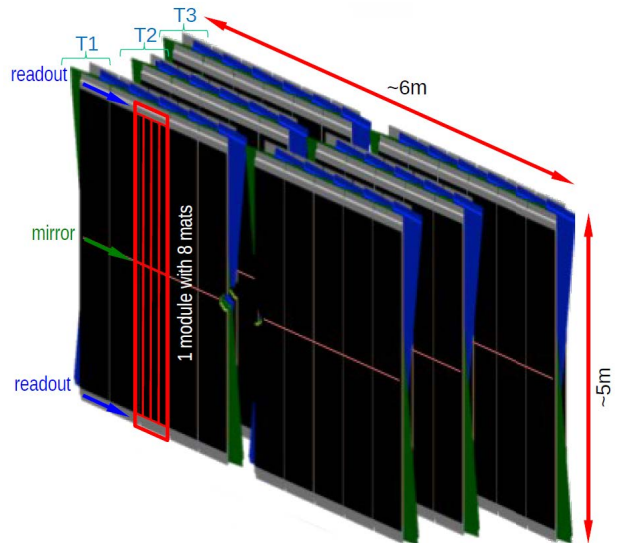
\includegraphics[width=0.9\textwidth]{logos/scifi.png}
        \caption{Visualization of the SciFi tracking stations.}
      \end{figure}
    \end{column}
    \begin{column}{0.48\textwidth}
      \begin{itemize}
        \item $\bullet$\, Consists of 3 stations (T1, T2, T3) with 4 layers each (X1, U, V, X2)
        \item $\bullet$\, Front two stations have 5 modules per side
        \item $\bullet$\, Back station has 6 modules on each side
        \item $\bullet$\, U, V layers have a $\mp 5 \deg$ stereo angle respectively
        \item $\bullet$\, \to\, used for determining y-position of track by comparing hitposition at different angles
      \end{itemize}
    \end{column}
  \end{columns}
\end{frame}

\begin{frame}\frametitle{SciFi terminology}
  \begin{columns}
    \begin{column}[c]{0.48\textwidth}
      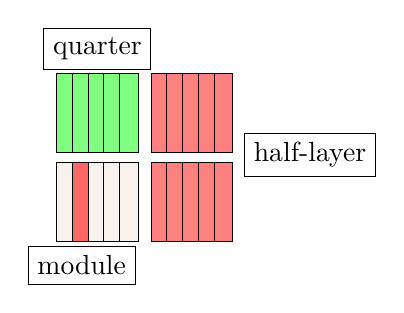
\begin{tikzpicture}
% first quarter
  \node[rectangle,
      draw = black,
      % text = ,
      fill = brown!10!white,
      minimum width = 0.2cm,
      minimum height = 1cm] (r) at (0,0) {};

  \node[rectangle,
      draw = black,
      % text = half-module,
      fill = red!60!white,
      minimum width = 0.2cm,
      minimum height = 1cm] (r) at (0.2,0) {};

  \node[rectangle,
      draw = black,
      % text = ,
      fill = brown!10!white,
      minimum width = 0.2cm,
      minimum height = 1cm] (r) at (0.4,0) {};

  \node[rectangle,
      draw = black,
      % text = ,
      fill = brown!10!white,
      minimum width = 0.2cm,
      minimum height = 1cm] (r) at (0.6,0) {};

  \node[rectangle,
      draw = black,
      % text = ,
      fill = brown!10!white,
      minimum width = 0.2cm,
      minimum height = 1cm] (r) at (0.8,0) {};

% second quarter
\node[rectangle,
    draw = black,
    % text = ,
    fill = red!50!white,
    minimum width = 0.2cm,
    minimum height = 1cm] (r) at (1.2,0) {};

\node[rectangle,
    draw = black,
    % text = ,
    fill = red!50!white,
    minimum width = 0.2cm,
    minimum height = 1cm] (r) at (1.4,0) {};

\node[rectangle,
    draw = black,
    % text = ,
    fill = red!50!white,
    minimum width = 0.2cm,
    minimum height = 1cm] (r) at (1.6,0) {};

\node[rectangle,
    draw = black,
    % text = ,
    fill = red!50!white,
    minimum width = 0.2cm,
    minimum height = 1cm] (r) at (1.8,0) {};

\node[rectangle,
    draw = black,
    % text = ,
    fill = red!50!white,
    minimum width = 0.2cm,
    minimum height = 1cm] (r) at (2,0) {};

% third quarter
\node[rectangle,
    draw = black,
    % text = ,
    fill = green!50!white,
    minimum width = 0.2cm,
    minimum height = 1cm] (r) at (0,1.13) {};

\node[rectangle,
    draw = black,
    % text = quarter,
    fill = green!50!white,
    minimum width = 0.2cm,
    minimum height = 1cm] (r) at (0.2,1.13) {};

\node[rectangle,
    draw = black,
    % text = ,
    fill = green!50!white,
    minimum width = 0.2cm,
    minimum height = 1cm] (r) at (0.4,1.13) {};

\node[rectangle,
    draw = black,
    % text = ,
    fill = green!50!white,
    minimum width = 0.2cm,
    minimum height = 1cm] (r) at (0.6,1.13) {};

\node[rectangle,
    draw = black,
    % text = ,
    fill = green!50!white,
    minimum width = 0.2cm,
    minimum height = 1cm] (r) at (0.8,1.13) {};

% fourth quarter
\node[rectangle,
    draw = black,
    % text = ,
    fill = red!50!white,
    minimum width = 0.2cm,
    minimum height = 1cm] (r) at (1.2,1.13) {};

\node[rectangle,
    draw = black,
    % text = ,
    fill = red!50!white,
    minimum width = 0.2cm,
    minimum height = 1cm] (r) at (1.4,1.13) {};

\node[rectangle,
    draw = black,
    % text = ,
    fill = red!50!white,
    minimum width = 0.2cm,
    minimum height = 1cm] (r) at (1.6,1.13) {};

\node[rectangle,
    draw = black,
    % text = ,
    fill = red!50!white,
    minimum width = 0.2cm,
    minimum height = 1cm] (r) at (1.8,1.13) {};

\node[rectangle,
    draw = black,
    % text = ,
    fill = red!50!white,
    minimum width = 0.2cm,
    minimum height = 1cm] (r) at (2,1.13) {};

\node[draw] at (0.4, 1.95) {quarter};
\node[draw] at (0.2, -0.8) {module};
\node[draw] at (3.1, 0.6) {half-layer};

\end{tikzpicture}

    \end{column}
    \begin{column}{0.48\textwidth}
      \begin{itemize}
        \item $\bullet$\, Long modules have the full height of the SciFi
        \item $\bullet$\, Half modules only span across one quarter
        \item $\bullet$\, layers are divided into two halves commonly labeled as A-side and C-side
        \begin{itemize}
          \item $\bullet$\, A-side: side from which the cavern is accessed
          \item $\bullet$\, C-side: side of the cryogenic lab
        \end{itemize}
        \item $\bullet$\, each layer can be split into four quarters, two per half layer
      \end{itemize}
    \end{column}
  \end{columns}
\end{frame}

\begin{frame}\frametitle{What is Alignment?}
  \begin{columns}
    \begin{column}[c]{0.48\textwidth}
      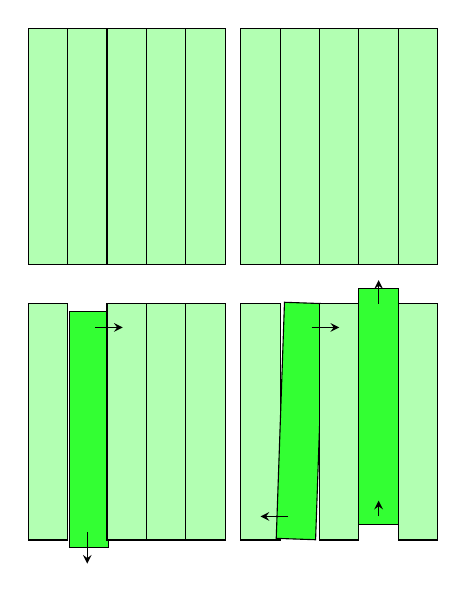
\begin{tikzpicture}
  % this is the ideal detector
  \node[rectangle,
      draw = black,
      % text = ,
      fill = green!30!white,
      minimum width = 0.5cm,
      minimum height = 3cm] (r) at (0,0) {};
  \node[rectangle,
      draw = black,
      % text = ,
      fill = green!80!white,
      minimum width = 0.5cm,
      minimum height = 3cm] (r) at (0.525,-0.1) {};
  \node[rectangle,
      draw = black,
      % text = ,
      fill = green!30!white,
      minimum width = 0.5cm,
      minimum height = 3cm] (r) at (1,0) {};
  \node[rectangle,
      draw = black,
      % text = ,
      fill = green!30!white,
      minimum width = 0.5cm,
      minimum height = 3cm] (r) at (1.5,0) {};
  \node[rectangle,
      draw = black,
      % text = ,
      fill = green!30!white,
      minimum width = 0.5cm,
      minimum height = 3cm] (r) at (2,0) {};

  \node[rectangle,
      draw = black,
      % text = ,
      fill = green!30!white,
      minimum width = 0.5cm,
      minimum height = 3cm] (r) at (2.7,0) {};
  \node[rectangle,
      draw = black,
      % text = ,
      fill = green!80!white,
      rotate around = {-2:(3.2,0)},
      minimum width = 0.5cm,
      minimum height = 3cm] (r) at (3.2,-0.1) {};
  % \draw (2.7,0) -- (5.7,0);
  \node[rectangle,
      draw = black,
      % text = ,
      fill = green!30!white,
      minimum width = 0.5cm,
      minimum height = 3cm] (r) at (3.7,0) {};
  \node[rectangle,
      draw = black,
      % text = ,
      fill = green!80!white,
      minimum width = 0.5cm,
      minimum height = 3cm] (r) at (4.2,0.2) {};
  \node[rectangle,
      draw = black,
      % text = ,
      fill = green!30!white,
      minimum width = 0.5cm,
      minimum height = 3cm] (r) at (4.7,0) {};

% now below it the physical detector
\node[rectangle,
    draw = black,
    % text = ,
    fill = green!30!white,
    minimum width = 0.5cm,
    minimum height = 3cm] (r) at (0,3.5) {};
\node[rectangle,
    draw = black,
    % text = ,
    fill = green!30!white,
    minimum width = 0.5cm,
    minimum height = 3cm] (r) at (0.5,3.5) {};
\node[rectangle,
    draw = black,
    % text = ,
    fill = green!30!white,
    minimum width = 0.5cm,
    minimum height = 3cm] (r) at (1,3.5) {};
\node[rectangle,
    draw = black,
    % text = ,
    fill = green!30!white,
    minimum width = 0.5cm,
    minimum height = 3cm] (r) at (1.5,3.5) {};
\node[rectangle,
    draw = black,
    % text = ,
    fill = green!30!white,
    minimum width = 0.5cm,
    minimum height = 3cm] (r) at (2,3.5) {};

\node[rectangle,
    draw = black,
    % text = ,
    fill = green!30!white,
    minimum width = 0.5cm,
    minimum height = 3cm] (r) at (2.7,3.5) {};
\node[rectangle,
    draw = black,
    % text = ,
    fill = green!30!white,
    minimum width = 0.5cm,
    minimum height = 3cm] (r) at (3.2,3.5) {};
\node[rectangle,
    draw = black,
    % text = ,
    fill = green!30!white,
    minimum width = 0.5cm,
    minimum height = 3cm] (r) at (3.7,3.5) {};
\node[rectangle,
    draw = black,
    % text = ,
    fill = green!30!white,
    minimum width = 0.5cm,
    minimum height = 3cm] (r) at (4.2,3.5) {};
\node[rectangle,
    draw = black,
    % text = ,
    fill = green!30!white,
    minimum width = 0.5cm,
    minimum height = 3cm] (r) at (4.7,3.5) {};

% draw arrows indicating the movement
% x and y translation
\draw [-stealth] (0.6,1.2) -- (0.95,1.2);
\draw [-stealth] (0.5,-1.4) -- (0.5,-1.8);

% rotation
\draw [-stealth] (3.35,1.2) -- (3.7,1.2);
\draw [-stealth] (3.05,-1.2) -- (2.7,-1.2);
% single translation
\draw [-stealth] (4.2,1.5) -- (4.2,1.8);
\draw [-stealth] (4.2,-1.2) -- (4.2,-1);

\end{tikzpicture}

    \end{column}
    \begin{column}[c]{0.48\textwidth}
      \begin{itemize}
        \item $\bullet$\, top: ideal detector, bottom: physical detector
        \item $\bullet$\, Surveys are used to find the rotation and position of each detector component
        \item $\bullet$\, Are used as starting positions for software alignment
      \end{itemize}
    \end{column}
  \end{columns}
\end{frame}

\begin{frame}\frametitle{The survey: what is it and the different types}
  \begin{columns}
    \begin{column}[c]{0.48\textwidth}
      \begin{itemize}
        \item $\bullet$\, measure distance of some points on the detector with a laser
        \item $\bullet$\, \to\, relative angles and positions between points are compared to simulation
      \end{itemize}
      \begin{figure}
        \centering
        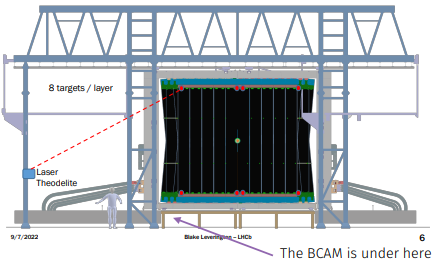
\includegraphics[width=0.7\textwidth]{logos/survey.png}
        % \caption{}
      \end{figure}
    \end{column}
    \begin{column}[c]{0.48\textwidth}
      \begin{itemize}
          \item $\bullet$\, 3 types:
          \item $\bullet$\, BCAM survey: over time, the BCAM monitors the positions of reference points on each layer
          \item $\bullet$\, module survey: performed inside assebly hall using reflective stickers keeping track of all positions
          \item $\bullet$\, layer survey: performed in the cavern on the layer in the front in closed state (both halves together)
      \end{itemize}
    \end{column}
  \end{columns}
\end{frame}

\begin{frame}\frametitle{Alignment: track fits with the Kalman Filter}
  \begin{columns}
    \begin{column}[c]{0.48\textwidth}
      \begin{figure}
        \centering
        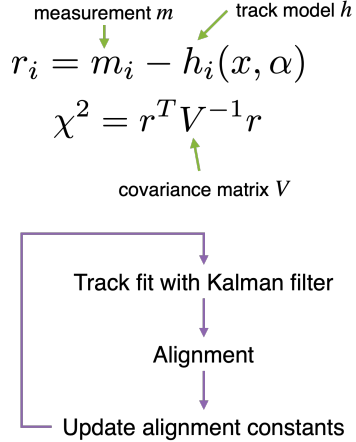
\includegraphics[width=0.72\textwidth]{logos/kalman.png}
        \caption{Alignment with Kalman Filter.}
      \end{figure}
    \end{column}
    \begin{column}[c]{0.48\textwidth}
      \begin{itemize}
        \item $\bullet$\, Use survey information as starting point
        \item $\bullet$\, Minimise $\chi^2$ with respect to the track parameters for the track fit
        \item $\bullet$\, Minimise $\chi^2$ with respect to the alignment parameters $\alpha$ during the alignment
        \item $\bullet$\, Update the alignment constants $\alpha$ and repeat until convergence criterium for $\chi^2$ is reached
        \item $\bullet$\, validate alignment quality using $\chi^2$
      \end{itemize}
    \end{column}
  \end{columns}
\end{frame}

\begin{frame}\frametitle{Alignment versions in use}
  \begin{columns}
    \begin{column}[c]{0.33\textwidth}
      \begin{itemize}
        \item V1:
        \item $\bullet$\, use full length modules
        \item $\bullet$\, alignable degrees of freedom: Tx Rz (x translation, rotation around z \to beam pipe axis)
      \end{itemize}
    \end{column}
    \begin{column}[c]{0.33\textwidth}
      \begin{itemize}
        \item low $\mu$:
        \item $\bullet$\, uses half modules
        \item $\bullet$\, uses VELO alignment on run 256145 data
        \item $\bullet$\, Tx Rz
      \end{itemize}
    \end{column}
    \begin{column}[c]{0.33\textwidth}
      \begin{itemize}
        \item V2:
        \item $\bullet$\, newest alignment version
        \item $\bullet$\, half modules (top half and bottom half)
        \item $\bullet$\, uses newest time alignment
        \item $\bullet$\, utilizes VELO alignment from run 256145
        \item $\bullet$\, used for HLT2 reprocessing
        \item $\bullet$\, $\mu \approx 2.26$ (run database)
      \end{itemize}
    \end{column}
  \end{columns}
\end{frame}

\begin{frame}\frametitle{Why analyse the quarters separately?}
  \begin{itemize}
    \item $\bullet$\, perfomance in each quarter might be very different from one another
    \item $\bullet$\, \to $\chi^2$ per quarter can provide more insights about the performance in each detector part
    \item $\bullet$\, v2 alignment shows improvements from v1 alignment but not across the whole SciFi
    \item $\bullet$\, find and resolve possible issues is easier
  \end{itemize}
  \to\, data from run 256145 is being used because at this point the current best alignment version v2 was in use
\end{frame}

\begin{frame}\frametitle{Hit distribution per quarter in V1 and V2 alignment}
  \begin{itemize}
    \item $\bullet$\, V1(left)- and V2(right) alignment on 20000 events with run 256145 data
    \item $\bullet$\, C-side: negative x direction, A-side: positive x
    \item $\bullet$\, plotted is x-coordinate against number of hits in each quarter coded by colour.
    \item $\bullet$\, 9 minimum hits per quarter (solid lines), 11 minimum hits (dashed lines)
  \end{itemize}
  \begin{figure}
    \subfloat[V1 alignment]{%
      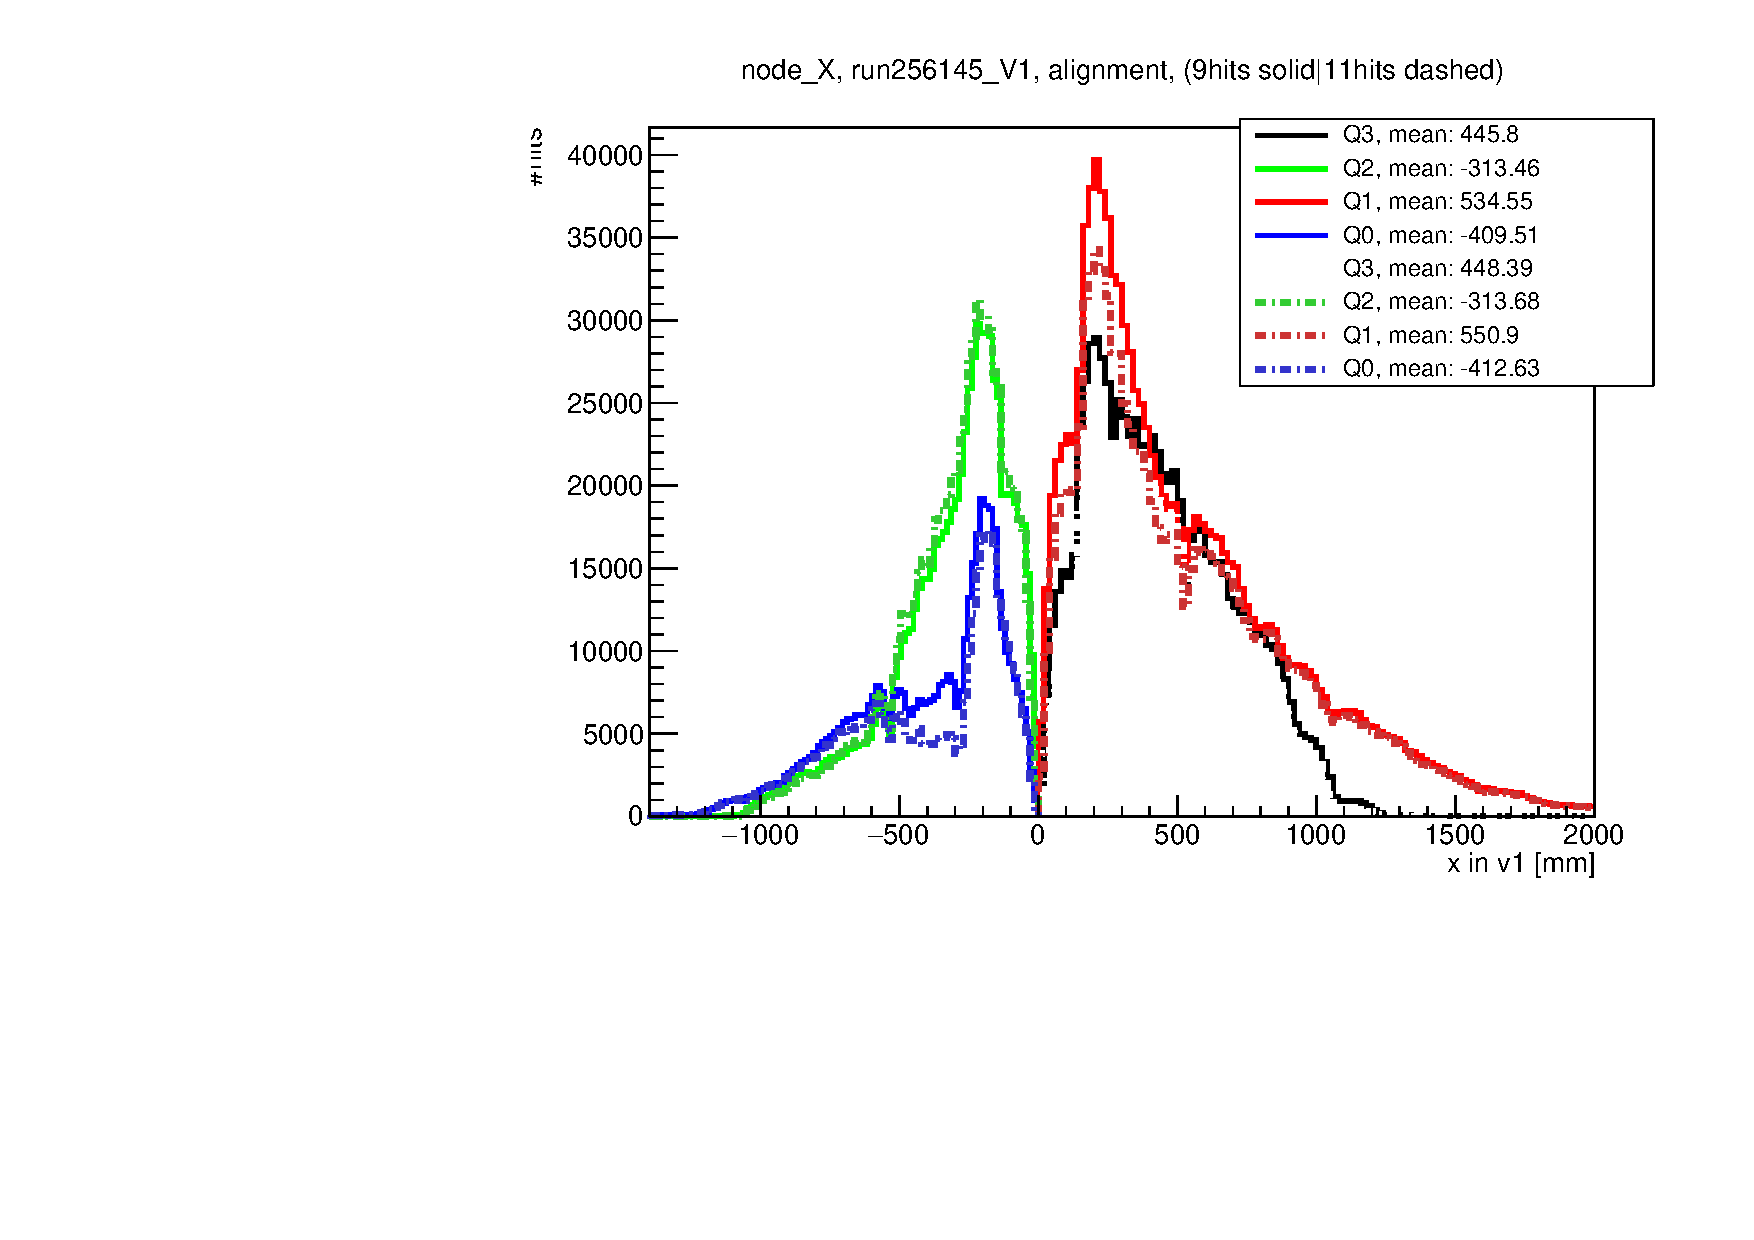
\includegraphics[width=0.45\textwidth]{compareHitNums/DataSeedsTupled_node_X_All_run256145_V1.pdf}%
    }
    \subfloat[V2 alignment]{%
      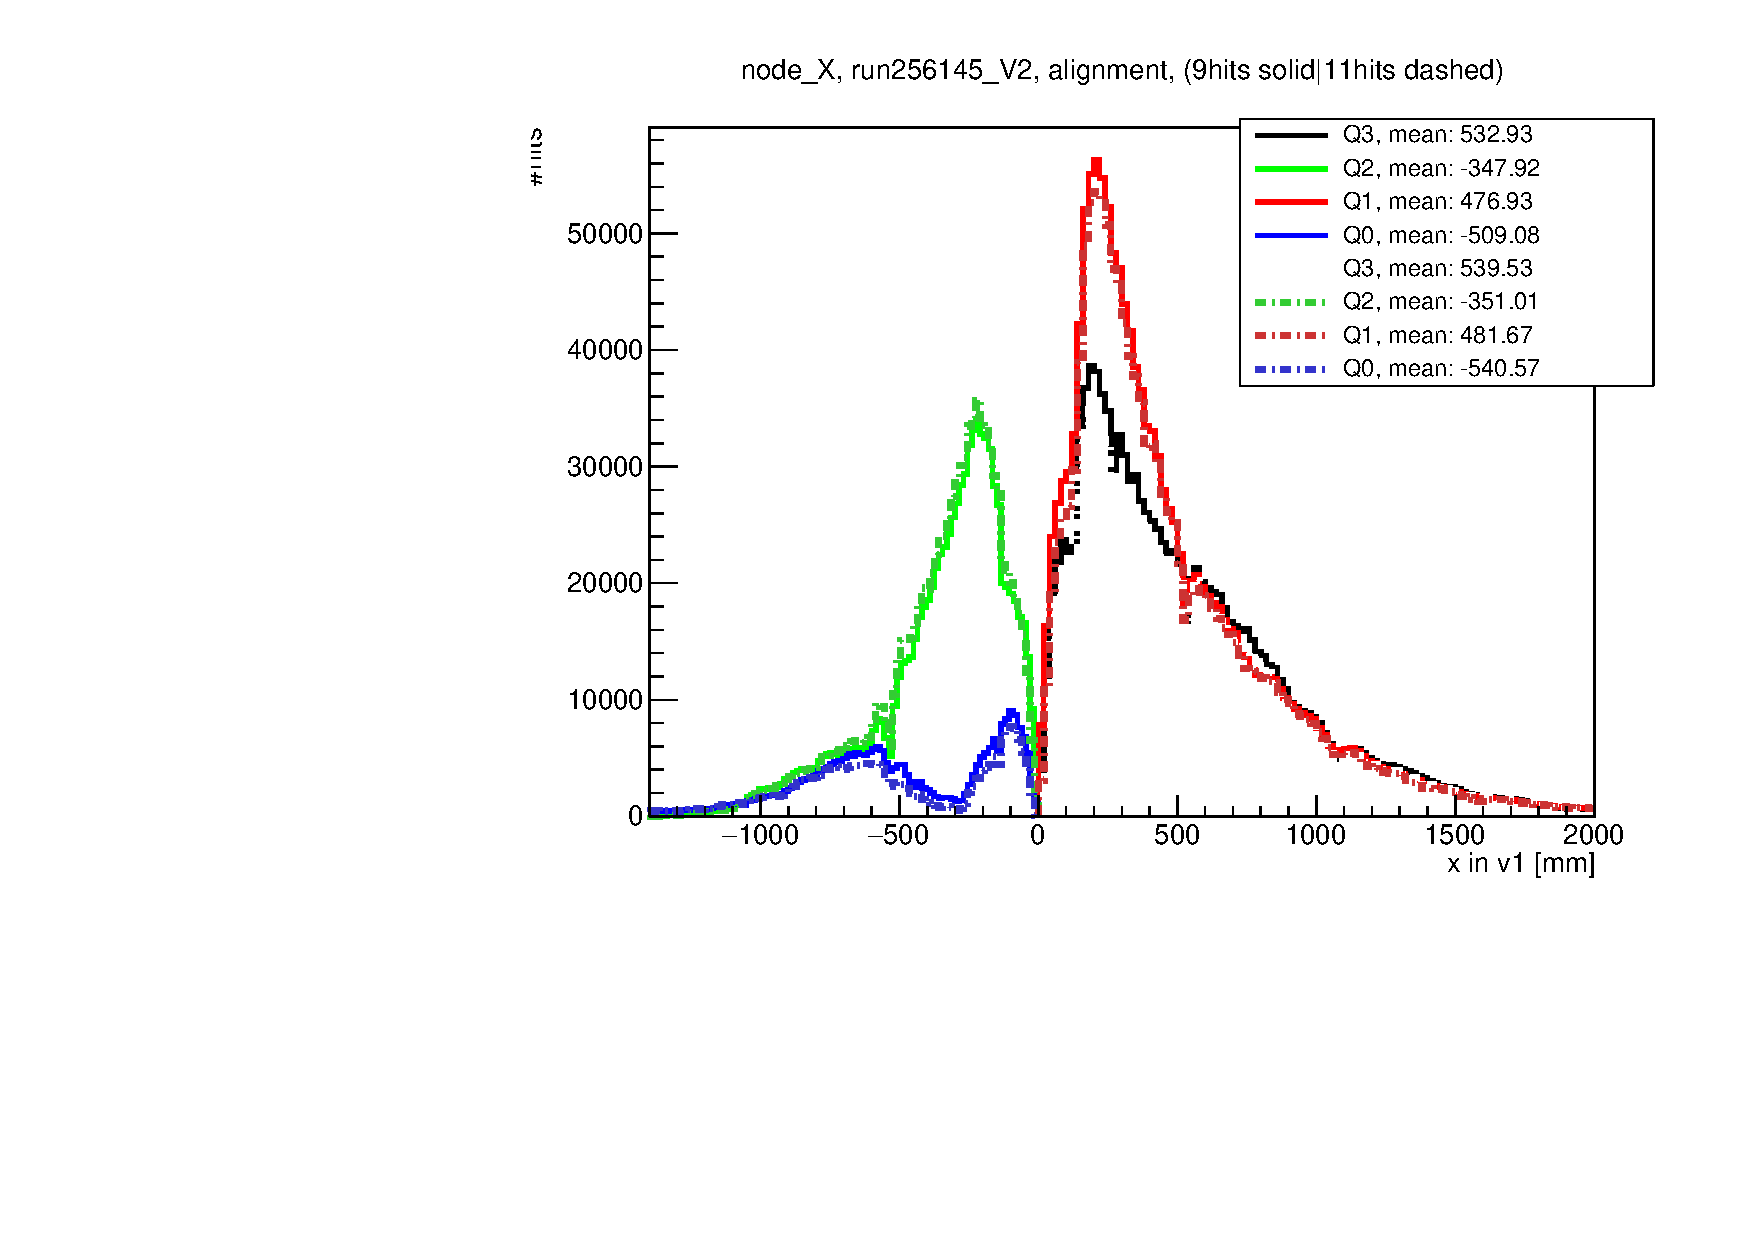
\includegraphics[width=0.45\textwidth]{compareHitNums/DataSeedsTupled_node_X_All_run256145_V2.pdf}%
    }
    % \caption{Hits on tracks in x-direction with run 256145 data on 20000 events using 9 minimum hits against 11 minimum hits.}
  \end{figure}
\end{frame}

% \begin{frame}\frametitle{Summary of Metrics from alignments in Quarter 0}
%   This hints that something is not right in Q0
%   \begin{columns}
%     \begin{column}[c]{0.48\textwidth}
%       \begin{figure}
%         \centering
%         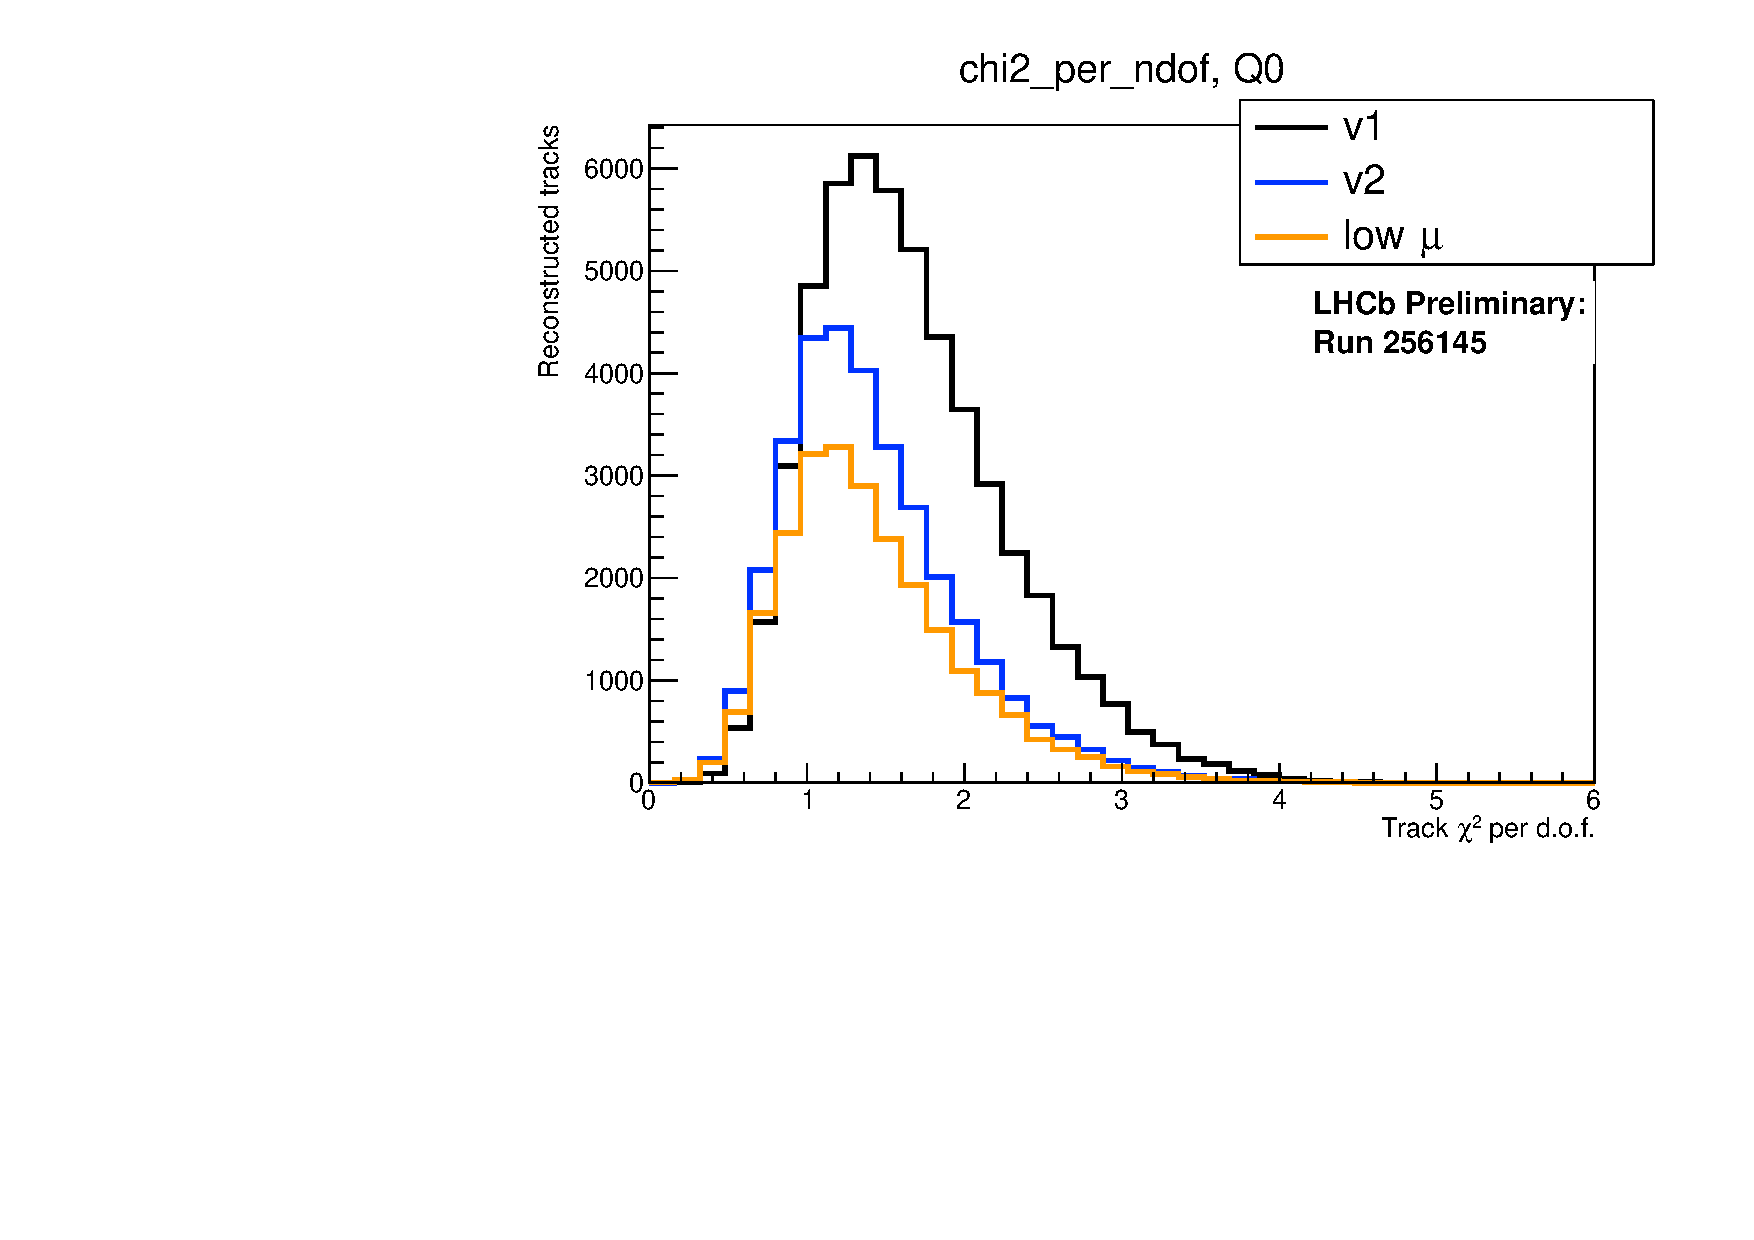
\includegraphics[width=0.9\textwidth]{2023-mar-9-DPG/chi2_per_ndof_Q0.pdf}
%         \caption{track $\chi^2$ per dof comparing each alignment for Quarter 0.}
%       \end{figure}
%     \end{column}
%     \begin{column}{0.48\textwidth}
%       \begin{figure}
%         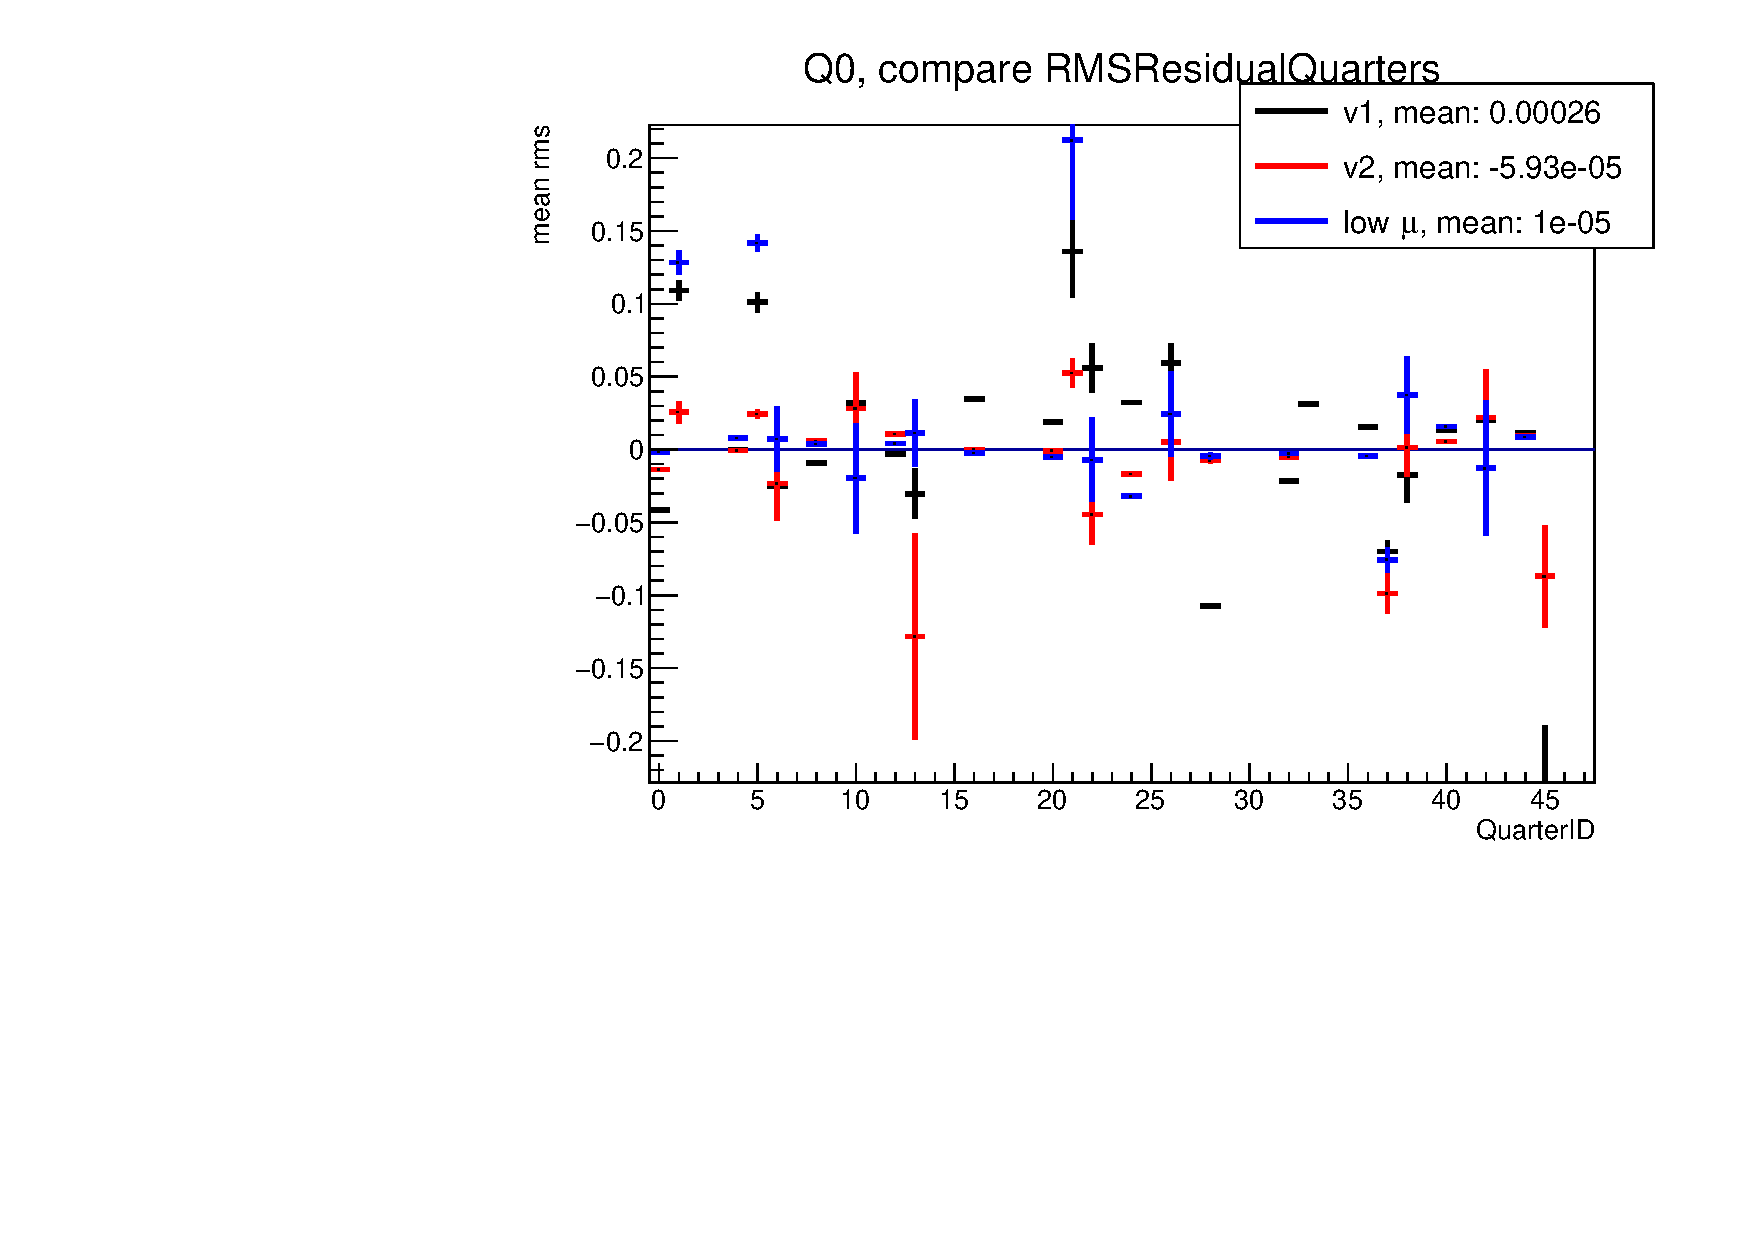
\includegraphics[width=0.9\textwidth]{2023-mar-9-DPG/RMSResidualQuarters_Q0.pdf}
%         \caption{Residual in each module for each alignment in Quarter 0.}
%       \end{figure}
%     \end{column}
%   \end{columns}
% \end{frame}

\begin{frame}\frametitle{Weighted residuals for V2 alignment}
    \begin{columns}
      \begin{column}[c]{0.48\textwidth}
        \begin{figure}
          \centering
          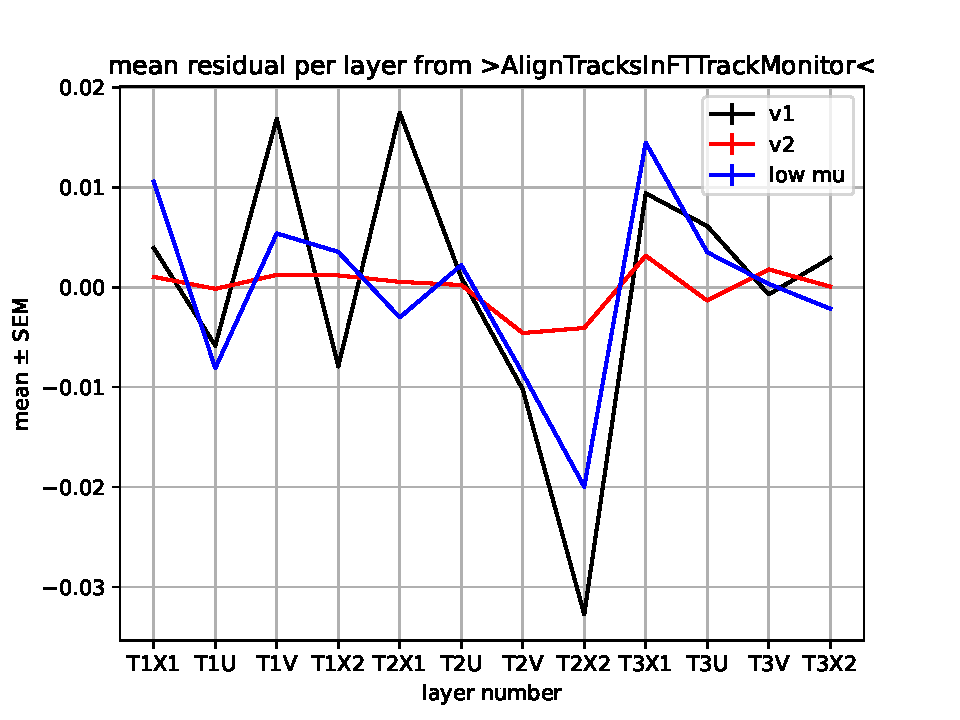
\includegraphics[width=0.7\textwidth]{2023-mar-9-DPG/meanResidual_AlignTracks_weighted.pdf}
          \caption{mean Residual per layer weighted with quarter hits.}
        \end{figure}
      \end{column}
      \begin{column}{0.48\textwidth}
        \begin{itemize}
          \item $\bullet$\, mean residual per quarter weighted: $
              \overline{\text{Res}_{L}} = \sum_{\text{layer}, \text{quarter}} \frac{\text{hits quarter of layer}}{\text{hits layer}}$
          \item $\bullet$\, goal: residual around 0 per layer
          \item $\bullet$\, V2 alignment shows overall improvement in alignment quality in every layer of the SciFi
          \item $\bullet$\, Investigating why T2X2 has a larger mean residual than any other layer
        \end{itemize}
      \end{column}
    \end{columns}
  \to\, V2 best performing alignment version for now, but still uses half modules
  \to\, long modules as in the physical SciFi preferred in the long run
\end{frame}

\begin{frame}\frametitle{Track hits comparison of alignment versions}
  \begin{columns}
    \begin{column}[c]{0.48\textwidth}
      \begin{itemize}
        \item $\bullet$\, V2 alignment with run 256145 data
        \item $\bullet$\, Hits on tracks as X-Y distribution with all layer information used
        \item $\bullet$\, C-side: negative x, A-side: positive x
        \item $\bullet$\, quite homogenous distribution of tracks throughout the whole A-side
        \item $\bullet$\, C-side tracks are not filled into the most outer modules
        \item $\bullet$\, information of all layers per quarter added on top of each other
        \item $\bullet$\, \to\, track distribution becomes clear looking at worst performing layer: T2X2
      \end{itemize}
    \end{column}
    \begin{column}[c]{0.48\textwidth}
      \begin{figure}
        \centering
        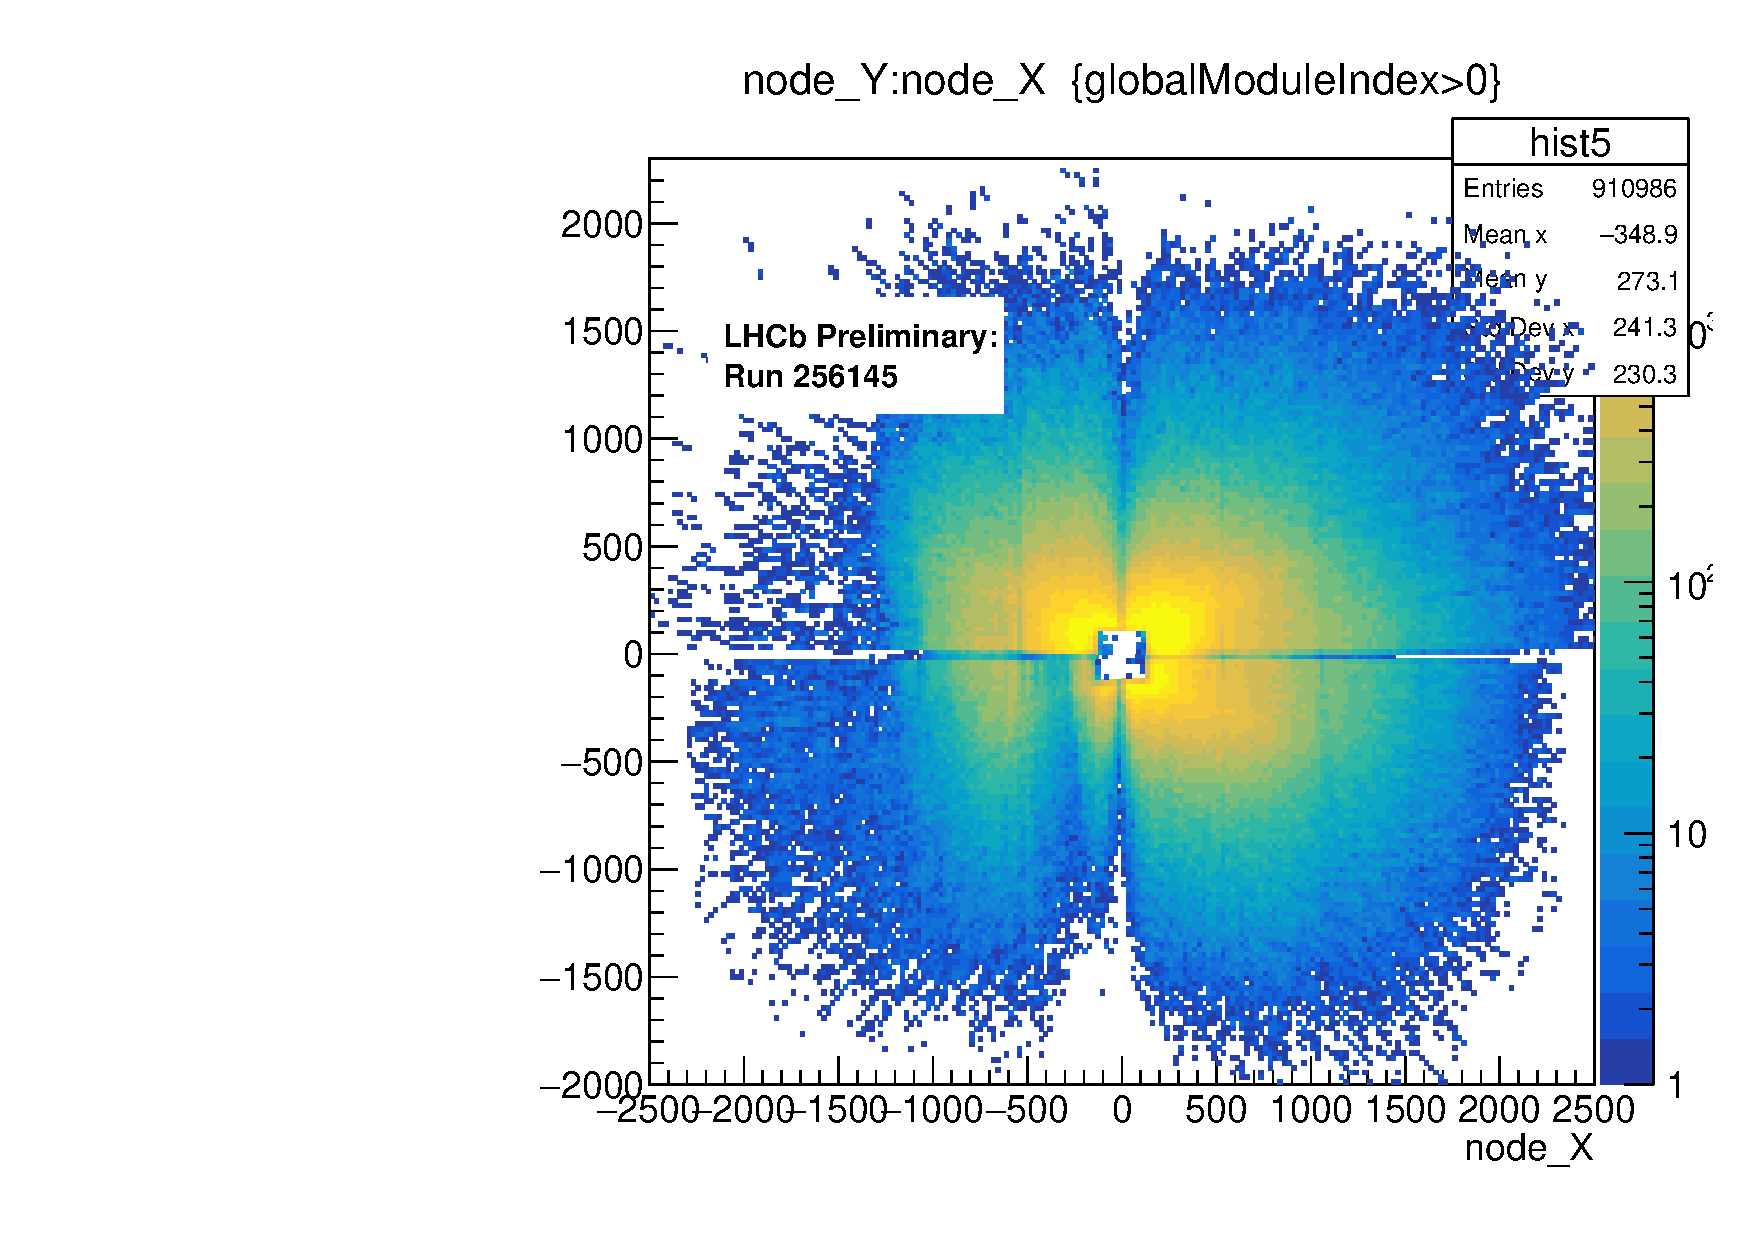
\includegraphics[width=0.9\textwidth]{tuples_out/combining_2D_nodeXY_v2.pdf}%
      \end{figure}
    \end{column}
  \end{columns}
\end{frame}

\begin{frame}\frametitle{New Q0 positions in T2X2 layer}
  \begin{itemize}
    \item $\bullet$\, changes based on V2 alignment positions
    \item $\bullet$\, manually scan rotations/positions of T2X2Q0 and register alignment tracks
    \item $\bullet$\, original V2 alignment has little to no tracks in Q0 because parts of the SciFi are too far out of alignment
    \item $\bullet$\, mean per quarter subtracted from V2 conditions xml in T2X2 now yielding tracks in M0 and M1
  \end{itemize}
  \begin{figure}
    \subfloat[]{%
      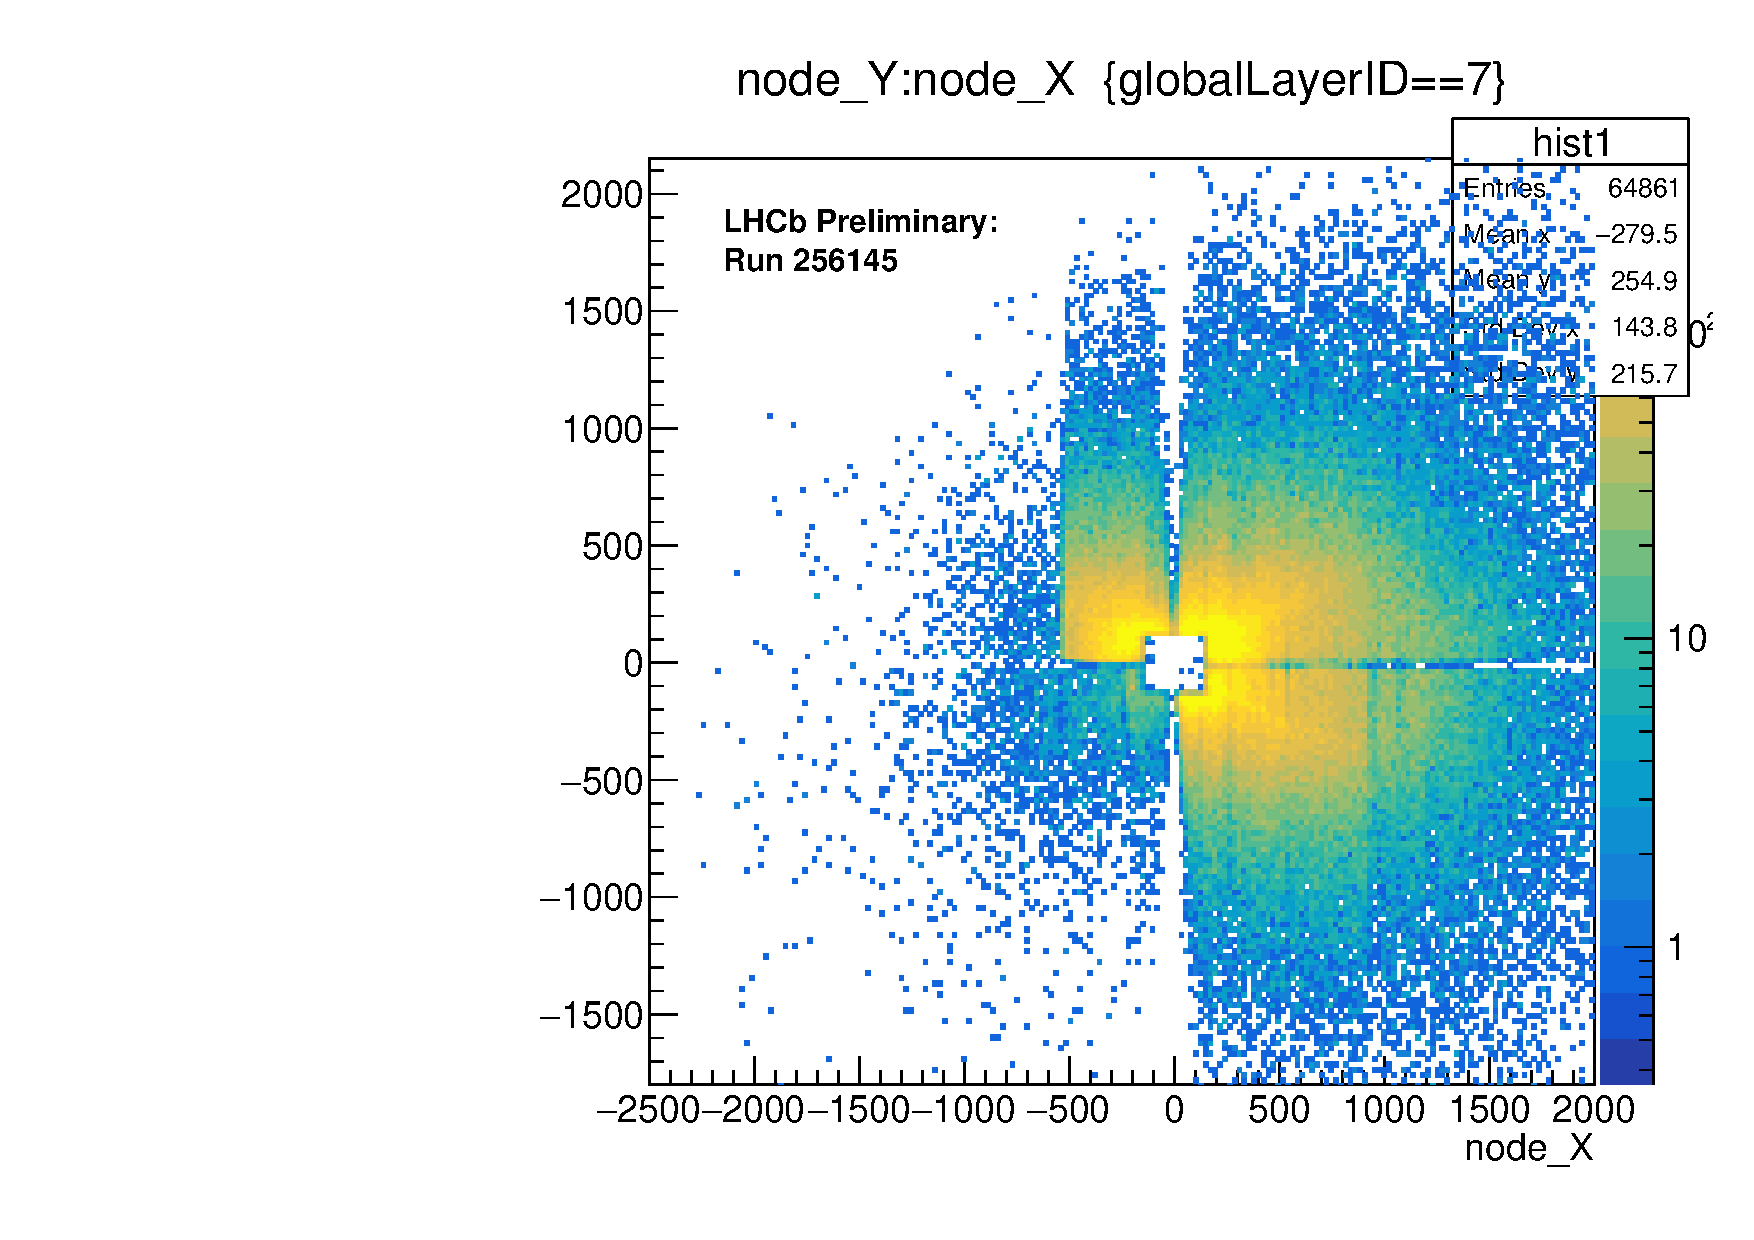
\includegraphics[width=0.28\textwidth]{2023-feb-07/v2_layers/2D_nodeXY_v2_7.pdf}%
    }
    \subfloat[]{%
      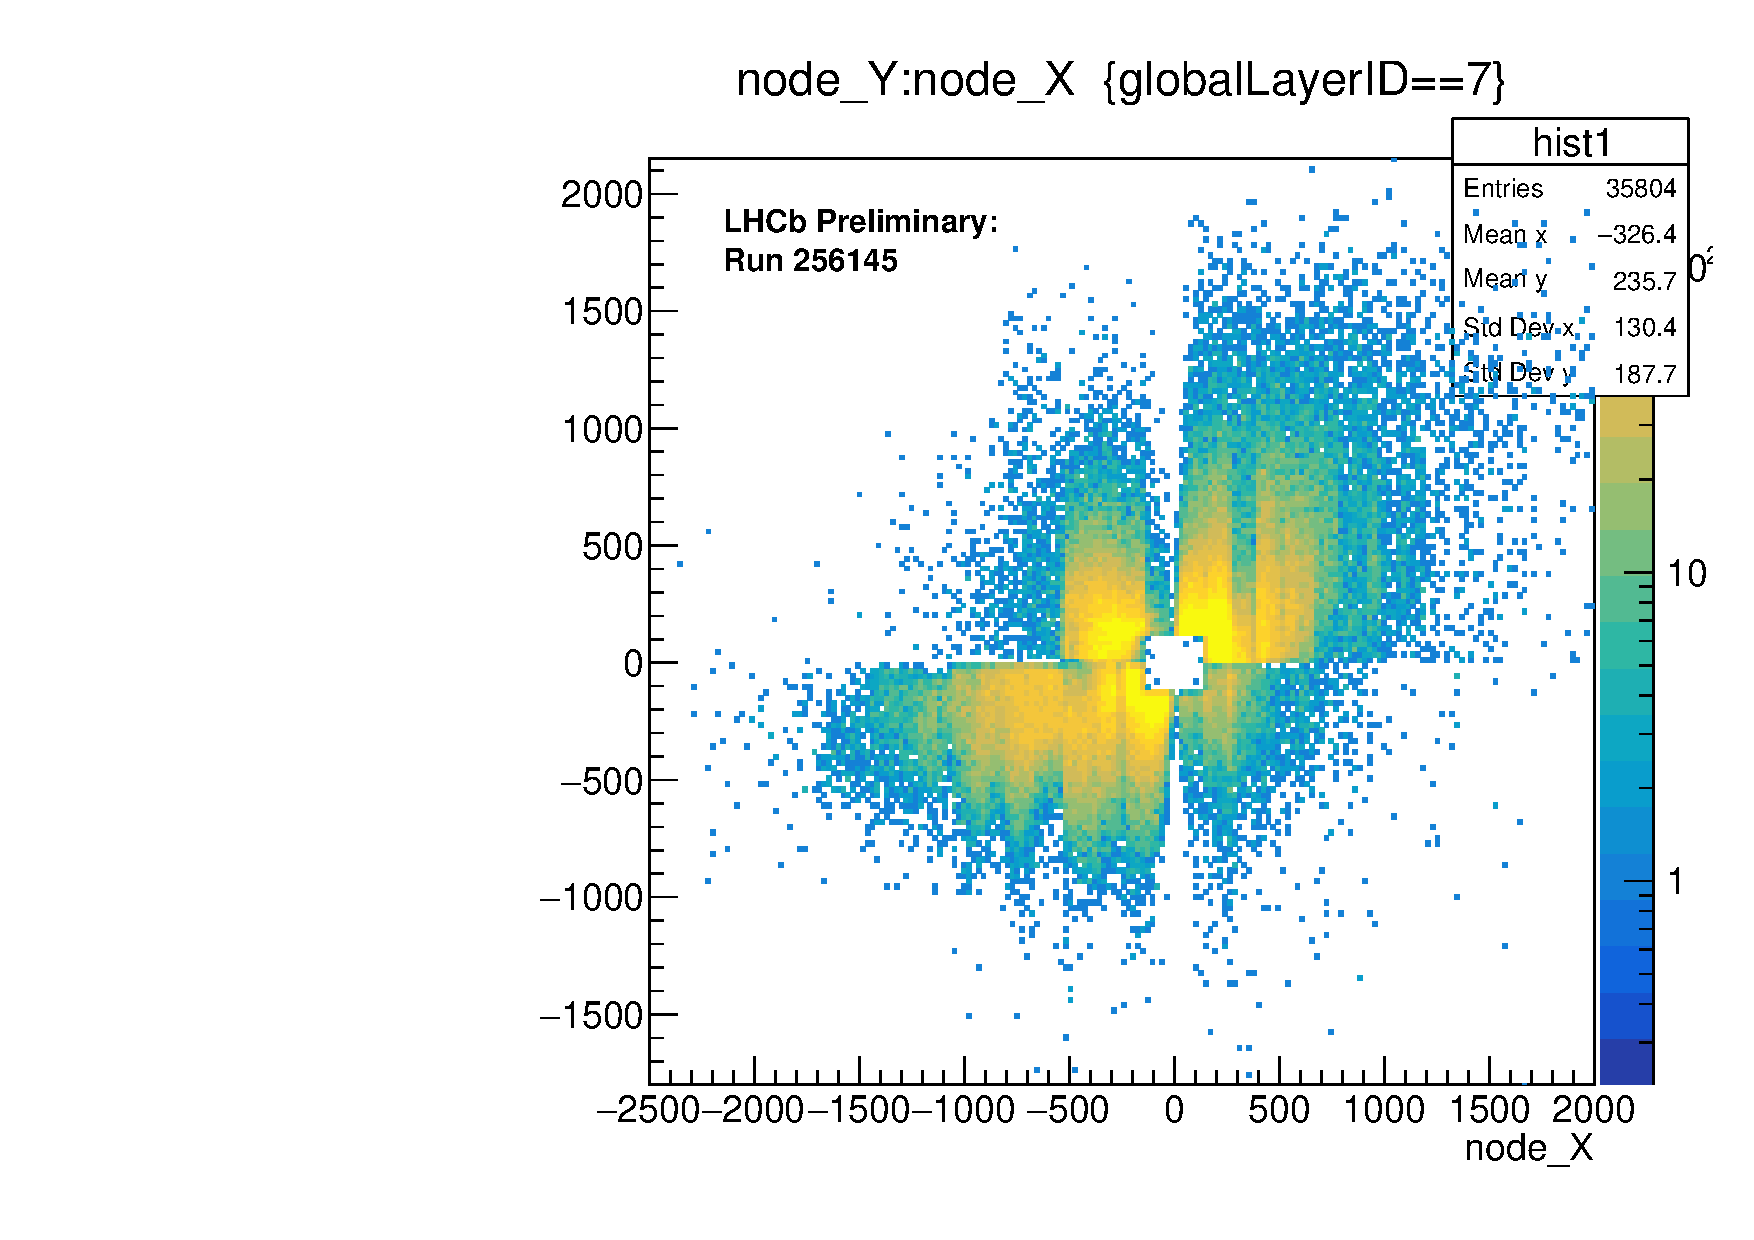
\includegraphics[width=0.28\textwidth]{2023-mar-9-DPG/extendedVars/2D_nodeXY_quartermean_7.pdf}%
    }
  \end{figure}
\end{frame}

\begin{frame}\frametitle{Summary}
  \begin{itemize}
    \item $\bullet$\, Trying to solve a puzzle with tracking alignment regarding C-side especially Quarter 0
    \item $\bullet$\, Source of complications: parts of the SciFi being too far out of alignment to be corrected
    \item $\bullet$\, \to\, An improvement of the alignment track hits in T2X2Q0 was achieved which results in more tracks in additional modules. Further investigation needed.
    \item $\bullet$\, A-side showed an improvement from V1 to V2
    \item $\bullet$\, Next steps:
    \item $\bullet$\, Test these starting condition in alignment + compare to current survey
    \item $\bullet$\, More investigation for T2X2Q2 as well configuration
  \end{itemize}
\end{frame}

\begin{frame}\frametitle{Sources}
  \begin{itemize}
    \item $\bullet$\,SciFi Conference Talk: \url{https://twiki.cern.ch/twiki/pub/LHCb/SciFiConference/fee_2018.pdf}
    \item $\bullet$\,LHCb SciFi: From performance requirements to an operational detector: \url{https://indico.cern.ch/event/1163878/}
    \item $\bullet$\, BCAM \url{https://accelconf.web.cern.ch/ipac2018/papers/wepaf067.pdf}
  \end{itemize}
\end{frame}

\end{document}
